\documentclass[xetex,mathserif,serif,aspectratio=169]{beamer}

\usepackage{xltxtra}
\usepackage{color}
\usepackage{url}
\usepackage{listings}
\usepackage{fontspec}
\usepackage{geometry}
\usepackage{lastpage}
\usepackage{fancyhdr}
\usepackage{amsmath}
\usepackage{amsthm}
\usepackage{amssymb}
\usepackage{blkarray}
\usepackage{multicol}
\usepackage{relsize}
\usepackage{listings}
\usepackage{xunicode}
\usepackage{xltxtra}
\usepackage{color}
\usepackage{url}
\usefonttheme[onlymath]{serif}

\definecolor{solarized@base03}{HTML}{002B36}
\definecolor{solarized@base02}{HTML}{073642}
\definecolor{solarized@base01}{HTML}{586e75}
\definecolor{solarized@base00}{HTML}{657b83}
\definecolor{solarized@base0}{HTML}{839496}
\definecolor{solarized@base1}{HTML}{93a1a1}
\definecolor{solarized@base2}{HTML}{EEE8D5}
\definecolor{solarized@base3}{HTML}{FDF6E3}
\definecolor{solarized@yellow}{HTML}{B58900}
\definecolor{solarized@orange}{HTML}{CB4B16}
\definecolor{solarized@red}{HTML}{DC322F}
\definecolor{solarized@magenta}{HTML}{D33682}
\definecolor{solarized@violet}{HTML}{6C71C4}
\definecolor{solarized@blue}{HTML}{268BD2}
\definecolor{solarized@cyan}{HTML}{2AA198}
\definecolor{solarized@green}{HTML}{859900}
\definecolor{yaleblue}{HTML}{0E4C92}

\newcommand{\yellow}[1]{\textcolor{solarized@yellow}{#1}}
\newcommand{\orange}[1]{\textcolor{solarized@orange}{#1}}
\newcommand{\red}[1]{\textcolor{solarized@red}{#1}}
\newcommand{\magenta}[1]{\textcolor{solarized@magenta}{#1}}
\newcommand{\violet}[1]{\textcolor{solarized@violet}{#1}}
\newcommand{\blue}[1]{\textcolor{solarized@blue}{#1}}
\newcommand{\cyan}[1]{\textcolor{solarized@cyan}{#1}}
\newcommand{\green}[1]{\textcolor{solarized@green}{#1}}
\newcommand{\yblue}[1]{\textcolor{yaleblue}{#1}}
\newcommand{\base}[1]{\textcolor{solarized@base01}{#1}}


\defaultfontfeatures{Mapping=tex-text}
\hypersetup{pdfstartview={FitH}}

\newcommand{\old}[1]{\fontspec[Alternate=1,Ligatures={Common}]{Hoefler Text}\fontsize{18pt}{30pt}\selectfont #1}%
\newcommand{\oldA}[1]{\fontspec[Alternate=1,Ligatures={Common, Rare}]{Hoefler Text}\fontsize{12pt}{15pt}\selectfont #1}%
\newcommand{\oldB}[1]{\fontspec[Ligatures={Common}]{Didot}\fontsize{12pt}{15pt}\color{solarized@base02}\selectfont #1}%
\newcommand{\tfont}[1]{\fontspec[Alternate=1,Ligatures={Common}]{Hoefler Text}\fontsize{12pt}{20pt}\selectfont #1}%
\newcommand{\dfont}[1]{\fontspec[Ligatures={Common}]{Didot}\fontsize{12pt}{12pt}\selectfont #1}%

\setbeamerfont{title}{family=\old}
\setbeamerfont{author}{family=\tfont}%
\setbeamerfont{frametitle}{family=\oldA}
\setbeamerfont{date}{family=\dfont}

\setbeamertemplate{navigation symbols}{}
\setbeamertemplate{footline}[text line]{%
  \parbox{0.99\linewidth}{
    \normalsize\vspace*{-24pt}\hfill{\color{solarized@base00}\insertframenumber/\inserttotalframenumber}
  }
}


\setlength{\parindent}{0pt}
\setlength{\parskip}{12pt}

\setbeamercolor{structure}{bg=solarized@base3, fg=solarized@base02}
\setbeamercolor{titlelike}{fg=solarized@cyan}
\setbeamercolor{title}{fg=solarized@blue}
\setbeamercolor{subtitle}{fg=solarized@magenta}
\setbeamercolor{alerted text}{fg=orange}
\setbeamercolor{itemize}{fg=solarized@base02}
\setbeamercolor{background canvas}{bg=solarized@base3}
\setbeamercolor{enumerate subitem}{fg=solarized@base02}

\newcommand{\minimize}{\mathop{\mathrm{minimize}}}
\newcommand{\argmin}{\mathop{\mathrm{arg\,min}}}
\newcommand{\argmax}{\mathop{\mathrm{arg\,max}}}
\newcommand{\st}{\mathop{\mathrm{subject\,\,to}}}


\usepackage[]{algorithm2e}
\usepackage{../kbordermatrix}

\begin{document}

%%%%%%%%%%%%%%%%%%%%%%%%%%%%%%%%%%%%%%%%%%%%%%%%%%%
\begin{frame}[fragile] \frametitle{} \oldB \small

\vfill

{\fontsize{0.7cm}{0cm}\selectfont Lecture 05 \\\vspace{0.2cm} Additive Models}\\\vspace{0.5cm}
01 February 2016

\vspace{2cm}

\begin{minipage}{0.6\textwidth}
Taylor B. Arnold \\
Yale Statistics \\
STAT 365/665
\end{minipage}
\hfill
\begin{minipage}{0.3\textwidth}\raggedleft

\includegraphics[scale=0.3]{../yale-logo.png}
\end{minipage}%

\end{frame}

%%%%%%%%%%%%%%%%%%%%%%%%%%%%%%%%%%%%%%%%%%%%%%%%%%%
\begin{frame}[fragile] \frametitle{} \oldB \small

\begin{itemize}
\item Problem set notes:
\begin{itemize}
\item Problem set 1 is due on Friday at 1pm!
\item brute force okay for implementation question
\item can use other libraries in the prediction and data analysis questions
\item consider \textbf{FNN} (R) or or \textbf{sklearn.neighbors} (Python)
\end{itemize}
\item Office hours:
\begin{itemize}
\item Taylor Arnold -- Mondays, 13:00 - 14:15, HH 24, Office 206 (by appointment)
\item Elena Khusainova -- Tuesdays, 13:00-15:00, HH 24, Basement
\item Yu Lu -- Tuesdays, 19:00-20:30, HH 24, Basement
\item Jason Klusowski -- Thursdays, 19:00-20:30, HH 24
\end{itemize}
\item If you have any questions on the problem set, please ask or send
them prior to Thursday night
\end{itemize}

\end{frame}


%%%%%%%%%%%%%%%%%%%%%%%%%%%%%%%%%%%%%%%%%%%%%%%%%%%
\begin{frame}[fragile] \frametitle{} \oldB \small

\textbf{\yblue{Factors}}

\begin{align*}
\renewcommand{\kbldelim}{(}% Left delimiter
\renewcommand{\kbrdelim}{)}% Right delimiter
  \kbordermatrix{
    & \\
    & \text{Canada} \\
    & \text{USA} \\
    & \text{USA} \\
    & \text{Mexico} \\
    & \text{Canada} \\
    & \text{Canada} \\
    & \text{USA} \\
    & \vdots \\
    & \text{Mexico}
  } &\rightarrow
\renewcommand{\kbldelim}{(}% Left delimiter
\renewcommand{\kbrdelim}{)}% Right delimiter
  \kbordermatrix{
    & \text{Canada} & \text{Mexico} & \text{USA} \\
    & 1             & 0             & 0          \\
    & 0             & 0             & 1          \\
    & 0             & 0             & 1          \\
    & 0             & 1             & 0          \\
    & 1             & 0             & 0          \\
    & 1             & 0             & 0          \\
    & 0             & 0             & 1          \\
    & \vdots        & \vdots        & \vdots     \\
    & 0             & 1             & 0          \\
  }
\end{align*}

\end{frame}

%%%%%%%%%%%%%%%%%%%%%%%%%%%%%%%%%%%%%%%%%%%%%%%%%%%
\begin{frame}[fragile] \frametitle{} \oldB \small

\textbf{\yblue{Higher dimensional problems}}

So far, we have only considered non-parametric estimators where the predictor
variable $x_i$ is one dimensional. How can we extend this to higher dimensional
models?

\pause Well, the \magenta{knn} and \magenta{kernel smoother} estimators only depend on
the distance matrix between points. Our efficient computational methods breakdown
in higher dimensions, but the theoretical idea of these need no modification.

\end{frame}

%%%%%%%%%%%%%%%%%%%%%%%%%%%%%%%%%%%%%%%%%%%%%%%%%%%
\begin{frame}[fragile] \frametitle{} \oldB \small

\begin{center}
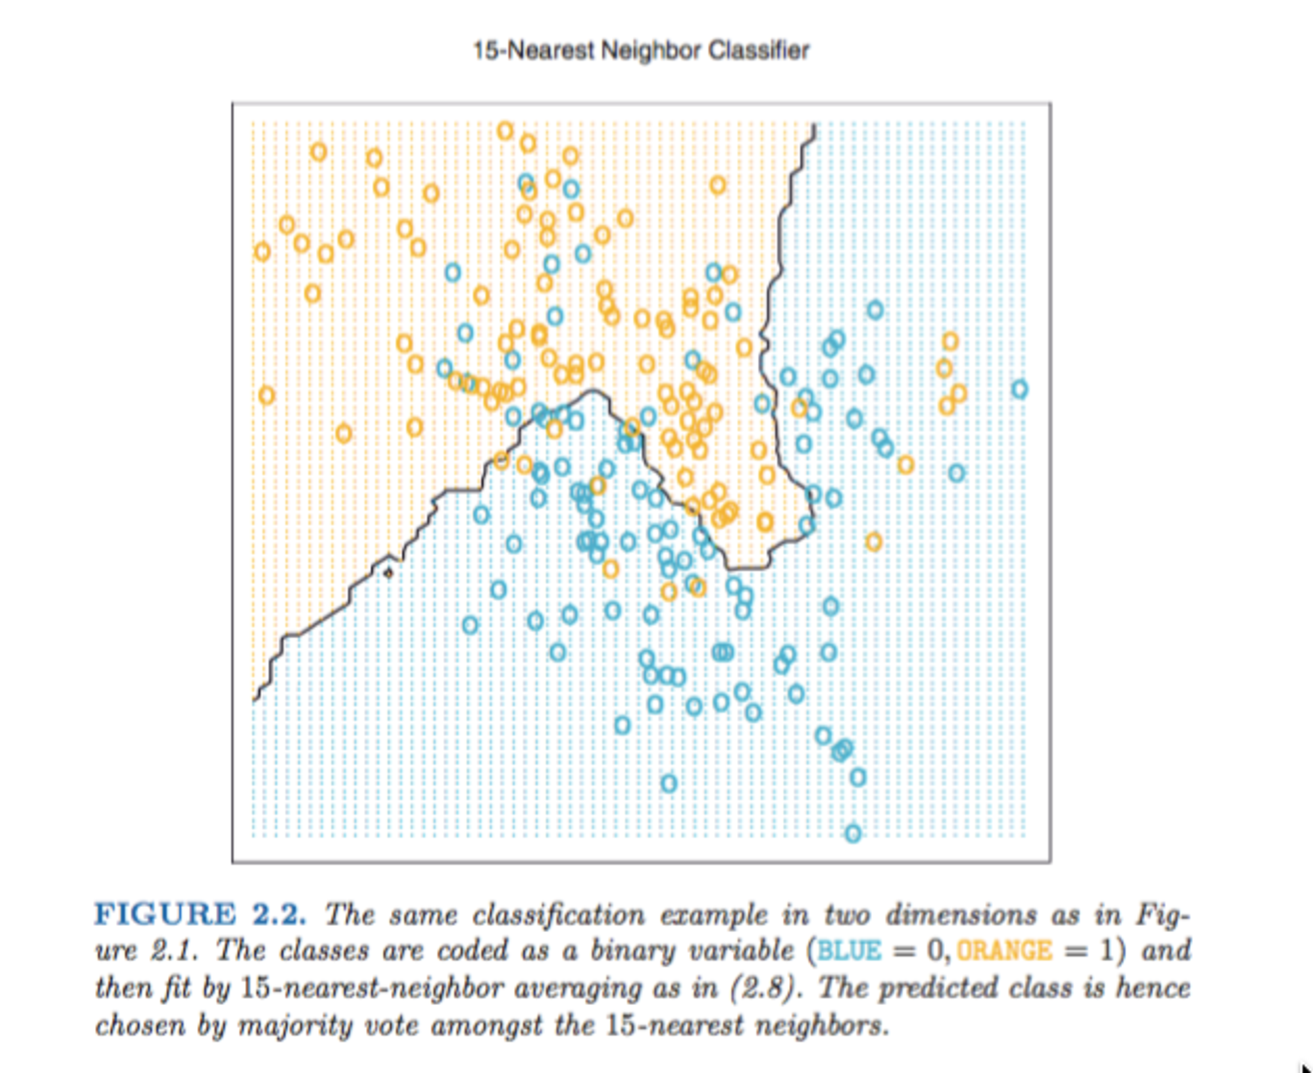
\includegraphics[width=0.7\textwidth]{img/pg15.pdf}
\end{center}

{\small \textbf{Elements of Statistical Learning, pg. 15}}

\end{frame}

%%%%%%%%%%%%%%%%%%%%%%%%%%%%%%%%%%%%%%%%%%%%%%%%%%%
\begin{frame}[fragile] \frametitle{} \oldB \small

\begin{center}
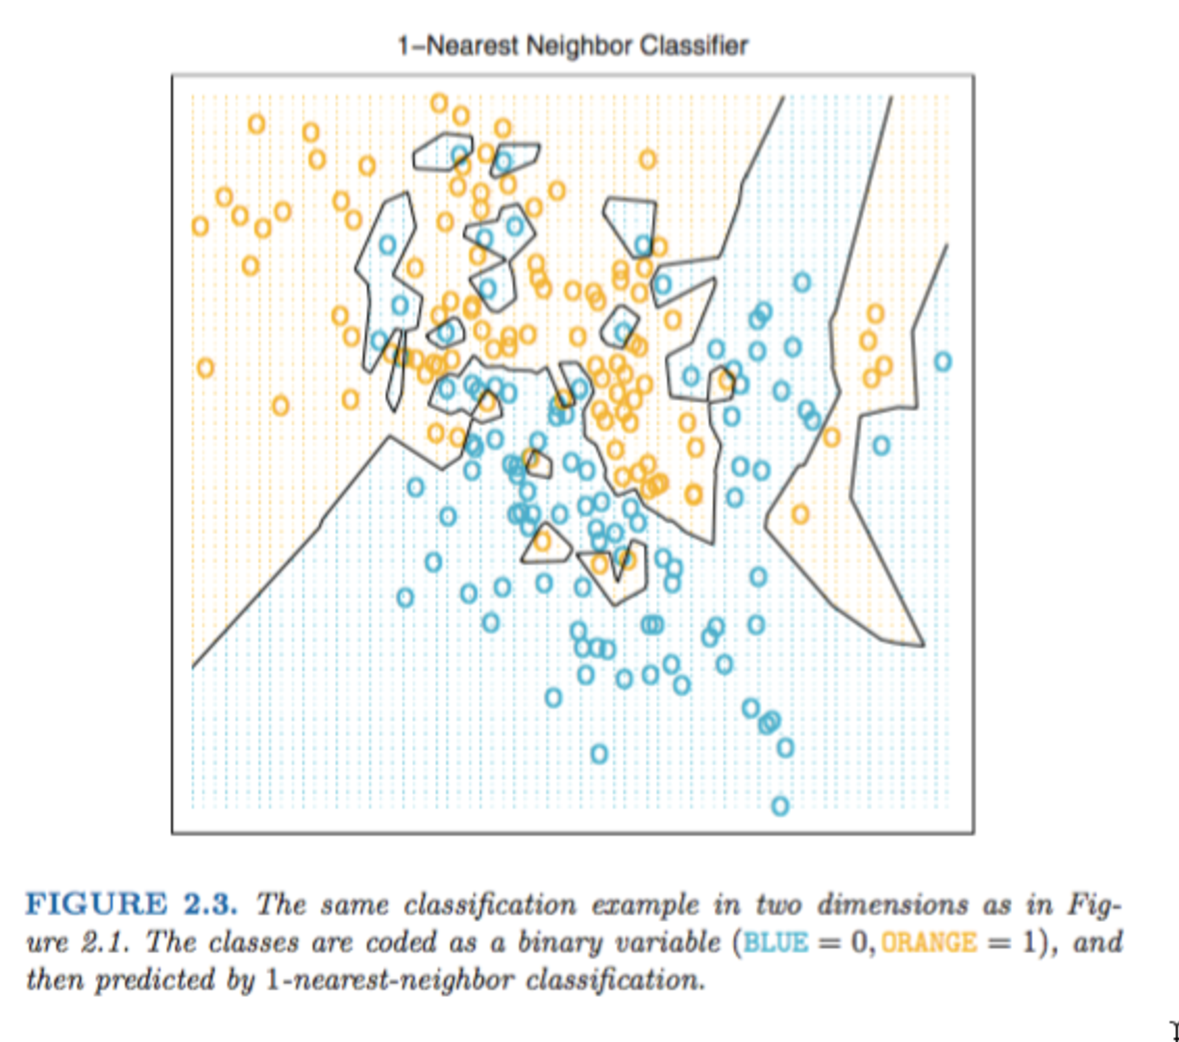
\includegraphics[width=0.7\textwidth]{img/pg16.pdf}
\end{center}

{\small \textbf{Elements of Statistical Learning, pg. 16}}

\end{frame}

%%%%%%%%%%%%%%%%%%%%%%%%%%%%%%%%%%%%%%%%%%%%%%%%%%%
\begin{frame}[fragile] \frametitle{} \oldB \small

\textbf{\yblue{Higher dimensional problems, cont.}}

What happens if we try to do basis expansion for linear regression in
higher dimensions?

\pause For clarity, let's assume we just have two dimensions labeled $x$ and $z$.
We need a basis that looks like:
\begin{align*}
y_i &= \sum_{j=0}^m \sum_{k=0}^m \beta_{j + m \cdot k} x_i^j z_i^k + \epsilon_i
\end{align*}
So the number of coordinates grows to $m^2$ coefficients in order to
fit arbitrary $m$ dimensional polynomials.

\pause For $p$ dimensions, we'll need a total $m^p$ coefficients; a quickly
unfeasible task. Regularization and keeping $m$ small can help, but still
makes this task hard for anything that would approximate a reasonably complex
non-linear surface.

\end{frame}

%%%%%%%%%%%%%%%%%%%%%%%%%%%%%%%%%%%%%%%%%%%%%%%%%%%
\begin{frame}[fragile] \frametitle{} \oldB \small

\textbf{\yblue{Higher dimensional problems, cont.}}

Lowess, local polynomial regression, can be fit in the same manor as the
linear model in higher dimensions. We can fix the order of the polynomial to
be $m=1$ while still capturing global non-linearity; therefore we can still
use this technique in higher dimensions.

\end{frame}

%%%%%%%%%%%%%%%%%%%%%%%%%%%%%%%%%%%%%%%%%%%%%%%%%%%
\begin{frame}[fragile] \frametitle{} \oldB \small

\textbf{\yblue{Additive models}}

One way to deal with the problem of basis expansion in higher dimensions
is to assume that there are no interaction between the variables. This
leads to a model such as:
\begin{align*}
y_i &= g_1(x_{i,1}) + g_2(x_{i,2}) + \cdots + g_p(x_{i,p})  + \epsilon_i
\end{align*}
These are known as \blue{additive models}.

\end{frame}

%%%%%%%%%%%%%%%%%%%%%%%%%%%%%%%%%%%%%%%%%%%%%%%%%%%
\begin{frame}[fragile] \frametitle{} \oldB \small

\textbf{\yblue{Additive models, cont.}}

Notice that the additive model cannot be defined uniquely as we can add a
constant to one of the $g_j(\cdot)$ functions and subtract the same constant from
another function $g_k(\cdot)$. In order to remedy this, one usually instead
writes an explicit intercept term:
\begin{align*}
y_i &= \alpha + g_1(x_{i,1}) + g_2(x_{i,2}) + \cdots + g_p(x_{i,p})  + \epsilon_i
\end{align*}
And constrains:
\begin{align*}
\sum_k g_k(x_{i,k}) &= 0
\end{align*}
For all values of $k$.

\end{frame}

%%%%%%%%%%%%%%%%%%%%%%%%%%%%%%%%%%%%%%%%%%%%%%%%%%%
\begin{frame}[fragile] \frametitle{} \oldB \small

\textbf{\yblue{Computing Additive models}}

The primary algorithm used for computing additive models is called
the \magenta{backfitting algorithm}. It was originally used for additive
models by Leo Breiman and Jerome Friedman:
\begin{quote}
Breiman, Leo, and Jerome H. Friedman. "Estimating optimal transformations for multiple regression and correlation." Journal of the American statistical Association 80.391 (1985): 580-598.
\end{quote}

\end{frame}

%%%%%%%%%%%%%%%%%%%%%%%%%%%%%%%%%%%%%%%%%%%%%%%%%%%
\begin{frame}[fragile] \frametitle{} \oldB \small

\textbf{\yblue{Computing Additive models, cont.}}

The algorithm can be compactly described as:
\begin{algorithm}[H]
 \KwData{pairs of data $\{(X_{i}, y_i)\}_{i=1}^n$}
 \KwResult{ Estimates $\widehat{\alpha}$ and $\widehat{g}_j$, $j = \{1, 2, \ldots, p\}$ }
 initialize $\widehat{\alpha} = \frac{1}{n} \sum_i y_i$, $\widehat{g}_j = 0$ \;
 \While{not converged}{
  \For{j=1 \emph{\KwTo} p}{
    $r_{ij} \leftarrow y_i - \widehat{a} - \sum_{k\neq j} \widehat{g}_k(x_{ik})$ \\
    $\widehat{g}_j \leftarrow \mathcal{S} \left(\left\{ (x_{ij}, r_{ij} ) \right\}_{i=1}^n\right)$ \\
    $\widehat{g}_j \leftarrow \widehat{g}_j - \frac{1}{n} \sum_i \widehat{g}_j(x_{ij}) $
  }
 }
\end{algorithm}
For some smoother function $\mathcal{S}$ and stopping criterion.

\end{frame}

%%%%%%%%%%%%%%%%%%%%%%%%%%%%%%%%%%%%%%%%%%%%%%%%%%%
\begin{frame}[fragile] \frametitle{} \oldB \small

\textbf{\yblue{Computing Additive models, cont.}}

For the smoothing function $\mathcal{S}$, we can use any of the algorithms we have already
studied. Local polynomial regression is a popular choice.

\pause Notice that we can also blend the additive model with higher dimensional
smoothers, particularly if we know that a small set of variables may have interactions
with each other even though most variables do not:
\begin{align*}
y_i &= \alpha + g_1(x_{i,1},x_{i,2}) + g_3(x_{i,3}) +  \cdots + g_p(x_{i,p})  + \epsilon_i.
\end{align*}

\end{frame}

%%%%%%%%%%%%%%%%%%%%%%%%%%%%%%%%%%%%%%%%%%%%%%%%%%%
\begin{frame}[fragile] \frametitle{} \oldB \small

\textbf{\yblue{Computing Additive models, cont.}}

There are two popular R packages for fitting additive
models. Either \textbf{mgcv}:
\begin{quote}
\url{https://cran.r-project.org/web/packages/mgcv}
\end{quote}
Or \textbf{gam}:
\begin{quote}
\url{https://cran.r-project.org/web/packages/gam}
\end{quote}

\pause There are not as many options for python. The best
I know of is in \textbf{statsmodels.sandbox.gam} as
\textit{AdditiveModel}.

\end{frame}

%%%%%%%%%%%%%%%%%%%%%%%%%%%%%%%%%%%%%%%%%%%%%%%%%%%
\begin{frame}[fragile] \frametitle{} \oldB \small

\textbf{\yblue{What's wrong with linear regression?}}

At this point you may wonder why linear regression seems to have trouble
in higher dimensions compared to the local methods. In truth, all of
these techniques have trouble with high dimensional spaces; it is just
that the others hide this fact in their definitions.

\pause The problem is the \magenta{curse of dimensionality}: When we have
high dimensional spaces, datasets look sparse even when the number of samples
is very large.

\pause Dealing with this is going to be the motivating problem in machine
learning for the remainder of the course.

\end{frame}

%%%%%%%%%%%%%%%%%%%%%%%%%%%%%%%%%%%%%%%%%%%%%%%%%%%
\begin{frame}[fragile] \frametitle{} \oldB \small

\begin{flushright}
{\color{yaleblue}\sc\fontsize{1cm}{0cm}\selectfont Data analysis}
\end{flushright}

\end{frame}


%%%%%%%%%%%%%%%%%%%%%%%%%%%%%%%%%%%%%%%%%%%%%%%%%%%
\begin{frame}[fragile] \frametitle{} \oldB \small

\textbf{\yblue{Description}}

Today we are going to look at housing price data, taking from
the American Community Survey and prepared by Cosma Shalizi:
\begin{quote}
\url{http://www.stat.cmu.edu/~cshalizi/uADA/13/hw/01/calif_penn_2011.csv}
\end{quote}
The data list aggregate statistics for census tracts.

\end{frame}

%%%%%%%%%%%%%%%%%%%%%%%%%%%%%%%%%%%%%%%%%%%%%%%%%%%
\begin{frame}[fragile] \frametitle{} \oldB \small

Let's first read in the data and look at all of the available
variables.
\begin{lstlisting}[language=R, basicstyle=\fontsize{8pt}{10pt}\selectfont\ttfamily]
> x <- read.csv("data/CAPA.csv", as.is=TRUE)
> names(x) <- tolower(names(x))
> str(x)
'data.frame': 11275 obs. of  34 variables:
 $ x                          : int  1 2 3 4 5 6 7 8 9 10 ...
 $ geo.id2                    : num  6e+09 6e+09 6e+09 6e+09 6e+09 ...
 $ statefp                    : int  6 6 6 6 6 6 6 6 6 6 ...
 $ countyfp                   : int  1 1 1 1 1 1 1 1 1 1 ...
 $ tractce                    : int  400100 400200 400300 400400 400500 ..
 $ population                 : int  2937 1974 4865 3703 3517 1571 4206 3594 2302 5678 ...
 $ latitude                   : num  37.9 37.8 37.8 37.8 37.8 ...
 $ longitude                  : num  -122 -122 -122 -122 -122 ...
 $ geo.display.label          : chr  "Census Tract 4001, Alameda County, California" ...
 $ median_house_value         : int  NA 909600 748700 773600 579200 439300 369800 ...
 $ total_units                : int  1425 929 2655 1911 1703 781 1977 1738 1202 2665 ...
 $ vacant_units               : int  162 37 134 68 71 65 236 257 80 500 ...
 $ median_rooms               : num  6.5 6 4.6 5 4.5 4.8 4.3 4.3 4.4 4.6 ...
\end{lstlisting}

\end{frame}

%%%%%%%%%%%%%%%%%%%%%%%%%%%%%%%%%%%%%%%%%%%%%%%%%%%
\begin{frame}[fragile] \frametitle{} \oldB \small

\begin{lstlisting}[language=R, basicstyle=\fontsize{8pt}{10pt}\selectfont\ttfamily]
 $ mean_household_size_owners : num  2.02 2.53 2.45 2.04 2.66 2.58 2.72 2.17 2.7 2.75 ...
 $ mean_household_size_renters: num  1.59 1.81 1.66 2.19 1.72 2.18 2.15 1.93 1.92 2.08 ...
 $ built_2005_or_later        : num  4.6 0 0 0 0 0 0 13.1 0 0 ...
 $ built_2000_to_2004         : num  9.3 1.2 0 0.2 0.2 0 0.6 4.1 2.2 2.2 ...
 $ built_1990s                : num  50.9 0 2.3 1.3 1.1 1.2 1.8 1.6 0.6 0 ...
 $ built_1980s                : num  2.5 1.3 3.2 0 1.9 1.4 2.2 2.4 5.9 0.5 ...
 $ built_1970s                : num  4.8 6.1 5.2 4.9 3.7 1 3.3 7.8 0 4.3 ...
 $ built_1960s                : num  1.3 6.5 8.3 4.3 5.8 6.5 0.8 3.7 5.5 11.2 ...
 $ built_1950s                : num  13.9 1 5.3 8 6 19.7 9.4 7.5 9.1 11.3 ...
 $ built_1940s                : num  2.8 10.8 7.8 10.4 7.5 17 9.7 13.3 14.7 8.5 ...
 $ built_1939_or_earlier      : num  9.9 73.2 68 71.1 73.8 53.1 72.4 46.5 62 62.1 ...
 $ bedrooms_0                 : num  3.6 3 11.5 5.2 4.9 3.5 8.2 8.9 14.2 6.1 ...
 $ bedrooms_1                 : num  5.6 16.4 28.4 27.7 30.2 20.4 22.3 25 20.1 29.3 ...
 $ bedrooms_2                 : num  11.9 27.4 29.2 33.7 38.1 40.1 43.2 37.5 39.4 35.4 ...
 $ bedrooms_3                 : num  40.6 34.4 20.4 21.9 19.3 30.7 16.7 25 18.3 25.3 ...
 $ bedrooms_4                 : num  31.6 17.5 7.9 7.3 5.4 4.6 6.5 2.1 5.5 3.9 ...
 $ bedrooms_5_or_more         : num  6.7 1.2 2.7 4.2 2.1 0.8 3.1 1.4 2.5 0 ...
 $ owners                     : num  81.2 66 45.1 45 43.6 51 32.2 28.3 31.7 35.1 ...
 $ renters                    : num  18.8 34 54.9 55 56.4 49 67.8 71.7 68.3 64.9 ...
 $ median_household_income    : int  156250 111667 66094 87306 62386 55658 40402 ...
 $ mean_household_income      : int  237805 195229 105877 106248 74604 73933 ...
\end{lstlisting}

\end{frame}

%%%%%%%%%%%%%%%%%%%%%%%%%%%%%%%%%%%%%%%%%%%%%%%%%%%
\begin{frame}[fragile] \frametitle{} \oldB \small

There are a few bad rows of data, but we can safely clean them
out:
\begin{lstlisting}[language=R, basicstyle=\fontsize{8pt}{10pt}\selectfont\ttfamily]
> badRows <- (apply(is.na(x),1,sum) != 0)
> table(badRows)
badRows
FALSE  TRUE
10605   670
> tapply(x$median_household_income, badRows, median, na.rm=TRUE)
 FALSE   TRUE
 55459 112813
> tapply(x$median_house_value, badRows, median, na.rm=TRUE)
 FALSE   TRUE
311100 516500
> tapply(x$vacant_units, badRows, median, na.rm=TRUE)
FALSE  TRUE
  107    70
> x <- na.omit(x)
\end{lstlisting}

\end{frame}

%%%%%%%%%%%%%%%%%%%%%%%%%%%%%%%%%%%%%%%%%%%%%%%%%%%
\begin{frame}[fragile] \frametitle{} \oldB \small

As you may have guessed from the file name, the housing
prices cover two distinct regions:
\begin{lstlisting}[language=R, basicstyle=\fontsize{8pt}{10pt}\selectfont\ttfamily]
> plot(x$longitude, x$latitude, pch=19, cex=0.5)
\end{lstlisting}

\end{frame}

%%%%%%%%%%%%%%%%%%%%%%%%%%%%%%%%%%%%%%%%%%%%%%%%%%%
\begin{frame}[fragile] \frametitle{} \oldB \small

\begin{center}
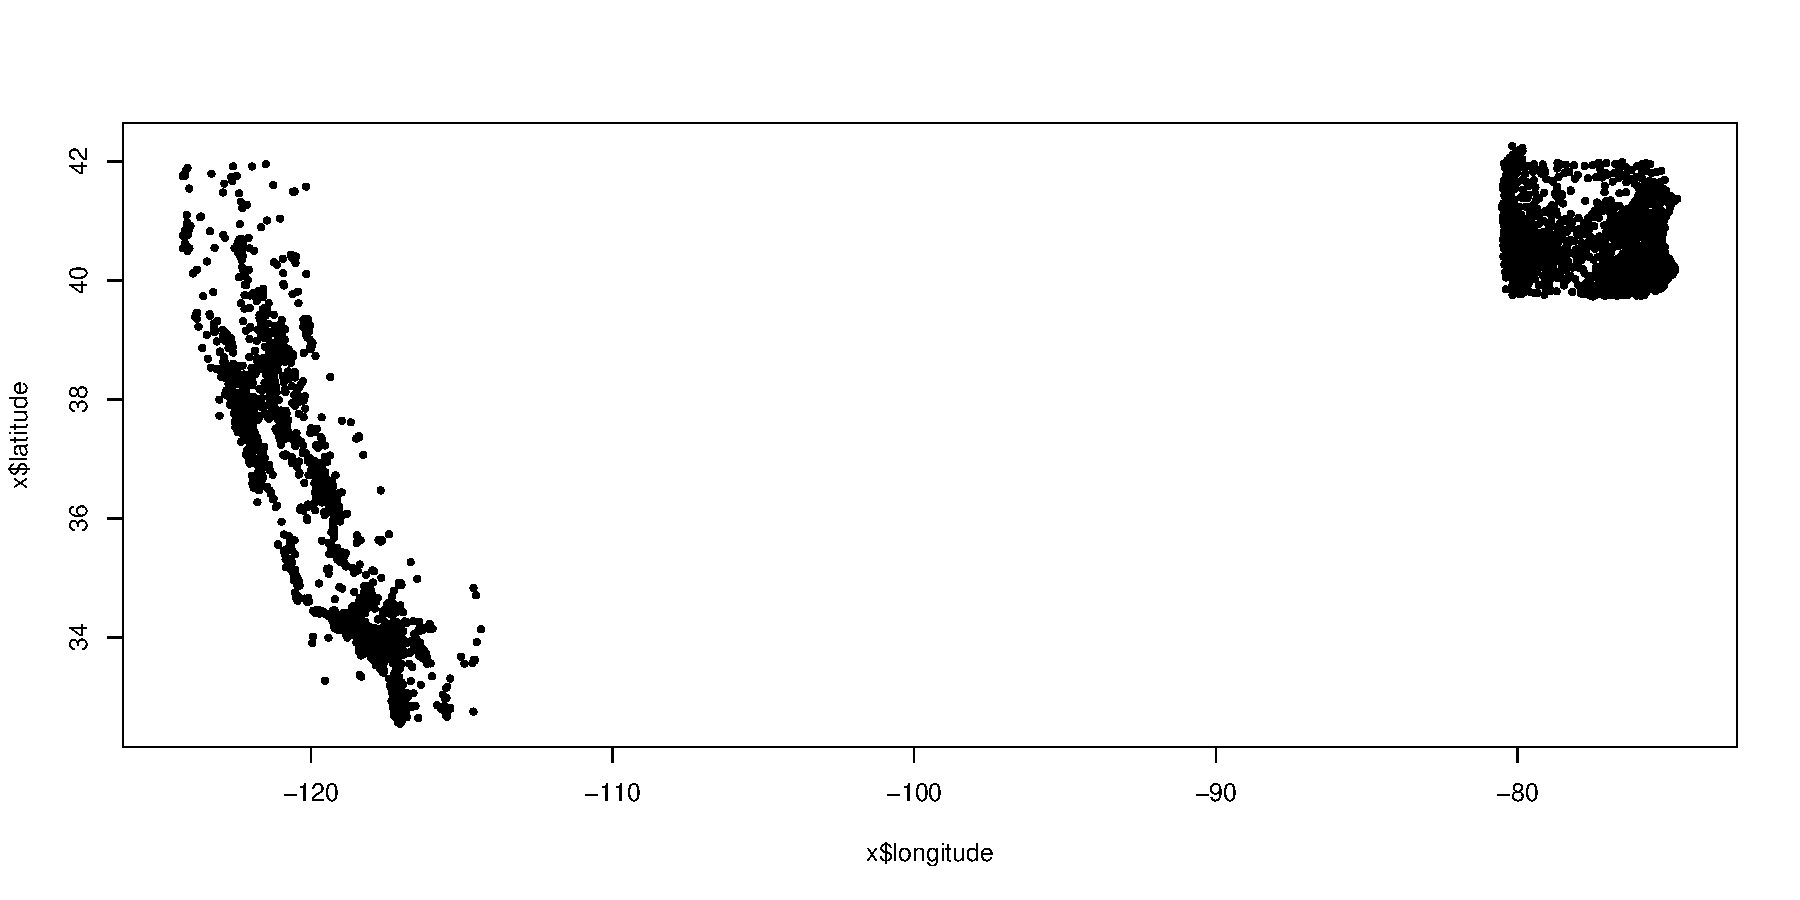
\includegraphics[width=\textwidth]{img/fig01.pdf}
\end{center}

\end{frame}

%%%%%%%%%%%%%%%%%%%%%%%%%%%%%%%%%%%%%%%%%%%%%%%%%%%
\begin{frame}[fragile] \frametitle{} \oldB \small

Let's split these two states up into two separate datasets.
I'll use the California set to start, but hopefully we will
have time to go back to the Pennsylvania set.
\begin{lstlisting}[language=R, basicstyle=\fontsize{8pt}{10pt}\selectfont\ttfamily]
> ca <- x[x$statefp==6,]
> pa <- x[x$statefp==42,]
\end{lstlisting}

\end{frame}

%%%%%%%%%%%%%%%%%%%%%%%%%%%%%%%%%%%%%%%%%%%%%%%%%%%
\begin{frame}[fragile] \frametitle{} \oldB \small

As a warm-up to additive models, let's fit and tune simple
knn model for whether the majority of residents in a census tract.
\begin{lstlisting}[language=R, basicstyle=\fontsize{8pt}{10pt}\selectfont\ttfamily]
> testFlag <- (runif(nrow(ca)) > 0.8)
> trainFlag <- !testFlag
> cl <- as.numeric(ca$owners < 50)
\end{lstlisting}
For the training set, we will use cross-validation to select
the optimal $k$:
\begin{lstlisting}[language=R, basicstyle=\fontsize{8pt}{10pt}\selectfont\ttfamily]
> X <- cbind(ca$latitude,ca$longitude)[trainFlag,]
> y <- cl[trainFlag]
> foldId <- sample(1:5,nrow(X),replace=TRUE)
\end{lstlisting}

\end{frame}

%%%%%%%%%%%%%%%%%%%%%%%%%%%%%%%%%%%%%%%%%%%%%%%%%%%
\begin{frame}[fragile] \frametitle{} \oldB \small

Here is the main validation code, using misclassification
error:
\begin{lstlisting}[language=R, basicstyle=\fontsize{8pt}{10pt}\selectfont\ttfamily]
> kvals <- 1:25
> res <- matrix(ncol=5, nrow=25)
> for (i in 1:5) {
+   trainSet <- which(foldId != i)
+   validSet <- which(foldId == i)
+   for (k in 1:25) {
+     pred <- knn(X[trainSet,],X[validSet,],y[trainSet],
+       k=kvals[k])
+     yhat <- (as.numeric(pred) - 1)
+     res[k,i] <- mean((y[validSet] != yhat))
+     print(k)
+   }
+ }
\end{lstlisting}

\end{frame}

%%%%%%%%%%%%%%%%%%%%%%%%%%%%%%%%%%%%%%%%%%%%%%%%%%%
\begin{frame}[fragile] \frametitle{} \oldB \small

Taking the results for each fold, I can calculate the
cross validated mis-classification rate as well as the
standard errors of these rates:
\begin{lstlisting}[language=R, basicstyle=\fontsize{8pt}{10pt}\selectfont\ttfamily]
> head(res)
     [,1] [,2] [,3] [,4] [,5]
[1,] 0.27 0.27 0.26 0.27 0.28
[2,] 0.23 0.25 0.23 0.25 0.27
[3,] 0.24 0.25 0.26 0.25 0.27
[4,] 0.22 0.23 0.24 0.25 0.25
[5,] 0.23 0.24 0.26 0.25 0.26
[6,] 0.23 0.24 0.24 0.26 0.25
> cvError <- apply(res,1,mean)
> cvSe <- apply(res,1,sd) / sqrt(5)
\end{lstlisting}

\end{frame}

%%%%%%%%%%%%%%%%%%%%%%%%%%%%%%%%%%%%%%%%%%%%%%%%%%%
\begin{frame}[fragile] \frametitle{} \oldB \small

\begin{center}
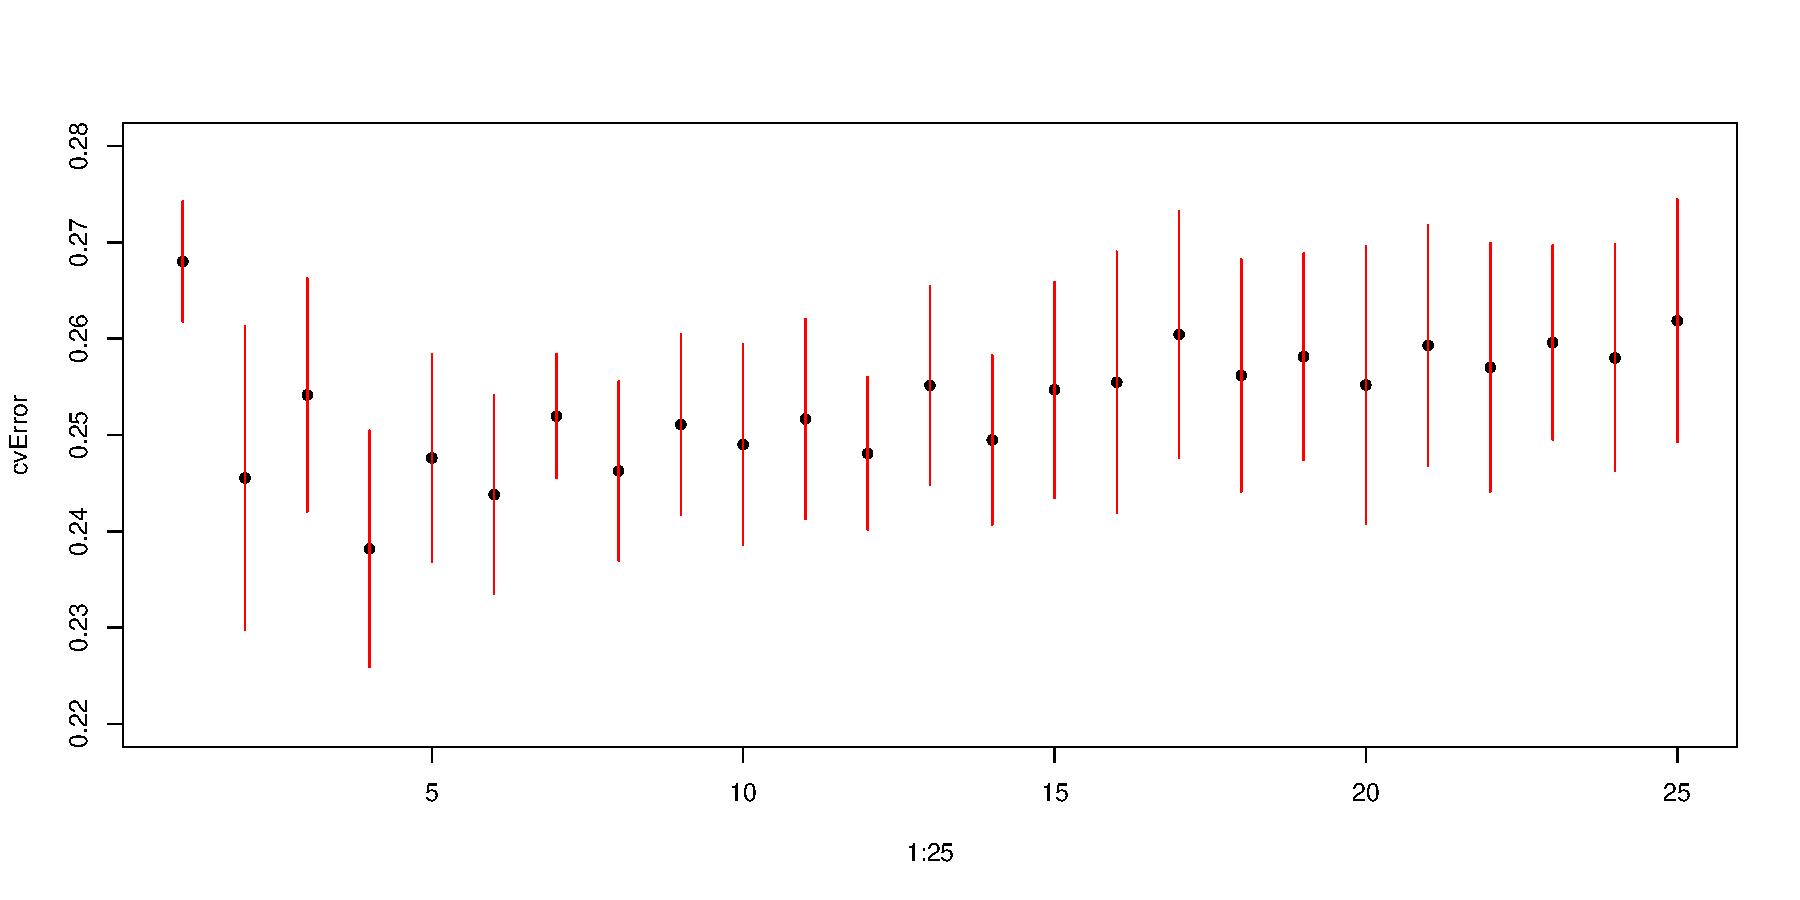
\includegraphics[width=\textwidth]{img/fig02.pdf}
\end{center}

\end{frame}

%%%%%%%%%%%%%%%%%%%%%%%%%%%%%%%%%%%%%%%%%%%%%%%%%%%
\begin{frame}[fragile] \frametitle{} \oldB \small

If we set the tuning parameter to $4$, we can then check
how well this performs on the test set.
\begin{lstlisting}[language=R, basicstyle=\fontsize{8pt}{10pt}\selectfont\ttfamily]
> Xtest <- cbind(ca$latitude,ca$longitude)[testFlag,]
> ytest <- cl[testFlag]
> yhat <- (as.numeric(knn(X,Xtest,y,k=4)) - 1)
> mean((yhat != ytest))
[1] 0.22
> round(table(yhat, ytest) / length(yhat) * 100)
    ytest
yhat  0  1
   0 56 16
   1  6 22
\end{lstlisting}
The table at the bottom is called a \blue{confusion matrix}, and
gives more granularity than the raw misclassification rate.

\end{frame}

%%%%%%%%%%%%%%%%%%%%%%%%%%%%%%%%%%%%%%%%%%%%%%%%%%%
\begin{frame}[fragile] \frametitle{} \oldB \small

If we set the tuning parameter to $4$, we can then check
how well this performs on the test set.
\begin{lstlisting}[language=R, basicstyle=\fontsize{8pt}{10pt}\selectfont\ttfamily]
> Xtest <- cbind(ca$latitude,ca$longitude)[testFlag,]
> ytest <- cl[testFlag]
> yhat <- (as.numeric(knn(X,Xtest,y,k=4)) - 1)
> mean((yhat != ytest))
[1] 0.22
> round(table(yhat, ytest) / length(yhat) * 100)
    ytest
yhat  0  1
   0 56 16
   1  6 22
\end{lstlisting}
The table at the bottom is called a \blue{confusion matrix}, and
gives more granularity than the raw misclassification rate.

\end{frame}

%%%%%%%%%%%%%%%%%%%%%%%%%%%%%%%%%%%%%%%%%%%%%%%%%%%
\begin{frame}[fragile] \frametitle{} \oldB \small

Now, I want to understand the variables that effect the
median house value in a census tract. Here is a linear
model that would be a good starting point (after some
exploratory plots, preferably):
\begin{lstlisting}[language=R, basicstyle=\fontsize{8pt}{10pt}\selectfont\ttfamily]
> ca.lm <- lm(log(median_house_value) ~ median_household_income
+  + mean_household_income + population + total_units +
+  + vacant_units + owners + median_rooms +
+  + mean_household_size_owners + mean_household_size_renters
+  + latitude + longitude, data = ca, subset=trainFlag)
\end{lstlisting}

\end{frame}


%%%%%%%%%%%%%%%%%%%%%%%%%%%%%%%%%%%%%%%%%%%%%%%%%%%
\begin{frame}[fragile] \frametitle{} \oldB \small

\begin{lstlisting}[language=R, basicstyle=\fontsize{8pt}{10pt}\selectfont\ttfamily]
> summary(ca.lm)
                             Estimate Std. Error t value Pr(>|t|)
(Intercept)                 -5.78e+00   5.93e-01   -9.74  < 2e-16 ***
median_household_income      1.20e-06   5.19e-07    2.30    0.021 *
mean_household_income        1.08e-05   4.35e-07   24.73  < 2e-16 ***
population                  -4.15e-05   5.59e-06   -7.42  1.3e-13 ***
total_units                  8.37e-05   1.73e-05    4.83  1.4e-06 ***
vacant_units                -1.06e-06   2.64e-05   -0.04    0.968
owners                      -3.83e-03   3.57e-04  -10.72  < 2e-16 ***
median_rooms                -1.49e-02   9.36e-03   -1.59    0.112
mean_household_size_owners   5.40e-02   7.99e-03    6.76  1.5e-11 ***
mean_household_size_renters -7.46e-02   7.20e-03  -10.36  < 2e-16 ***
latitude                    -2.15e-01   6.36e-03  -33.81  < 2e-16 ***
longitude                   -2.15e-01   6.67e-03  -32.29  < 2e-16 ***
---
Signif. codes:  0 ‘***’ 0.001 ‘**’ 0.01 ‘*’ 0.05 ‘.’ 0.1 ‘ ’ 1

Residual standard error: 0.32 on 5995 degrees of freedom
Multiple R-squared:  0.636, Adjusted R-squared:  0.635
F-statistic:  953 on 11 and 5995 DF,  p-value: <2e-16
\end{lstlisting}

\end{frame}

%%%%%%%%%%%%%%%%%%%%%%%%%%%%%%%%%%%%%%%%%%%%%%%%%%%
\begin{frame}[fragile] \frametitle{} \oldB \small

To fit an additive model in R, we can use the \texttt{mgcv}
package. It uses cross-validation by default, making it very
easy to use in place of linear regression.
\begin{lstlisting}[language=R, basicstyle=\fontsize{8pt}{10pt}\selectfont\ttfamily]
> library(mgcv)
Loading required package: nlme
This is mgcv 1.8-7. For overview type 'help("mgcv-package")'.
> ca.gam <- gam(log(median_house_value)
+   ~ s(median_household_income) + s(mean_household_income)
+   + s(population) + s(total_units) + s(vacant_units)
+   + s(owners) + s(median_rooms) + s(mean_household_size_owners)
+   + s(mean_household_size_renters) + s(latitude)
+   + s(longitude), data=ca, subset=trainFlag)
\end{lstlisting}

\end{frame}

%%%%%%%%%%%%%%%%%%%%%%%%%%%%%%%%%%%%%%%%%%%%%%%%%%%
\begin{frame}[fragile] \frametitle{} \oldB \small

To see the `coefficients' in the additive model, we
can plot the output object. These options work well
when working locally:
\begin{lstlisting}[language=R, basicstyle=\fontsize{8pt}{10pt}\selectfont\ttfamily]
> plot(ca.gam2,scale=0,se=2,shade=TRUE,resid=FALSE,pages=1)
\end{lstlisting}
For class, I add the option \texttt{select=i} to only
show the contribution of the $i$'th variable.

\end{frame}

%%%%%%%%%%%%%%%%%%%%%%%%%%%%%%%%%%%%%%%%%%%%%%%%%%%
\begin{frame}[fragile] \frametitle{} \oldB \small

\begin{center}
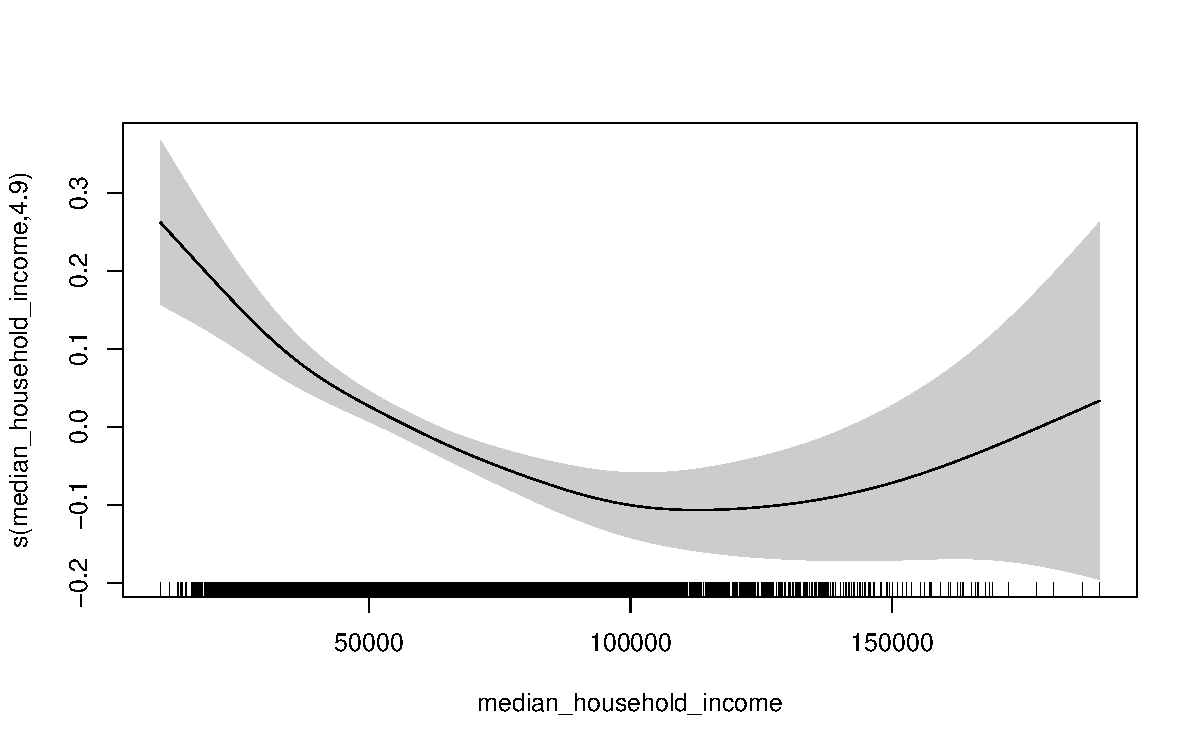
\includegraphics[width=\textwidth]{img/gamRug01.pdf}
\end{center}

\end{frame}

%%%%%%%%%%%%%%%%%%%%%%%%%%%%%%%%%%%%%%%%%%%%%%%%%%%
\begin{frame}[fragile] \frametitle{} \oldB \small

\begin{center}
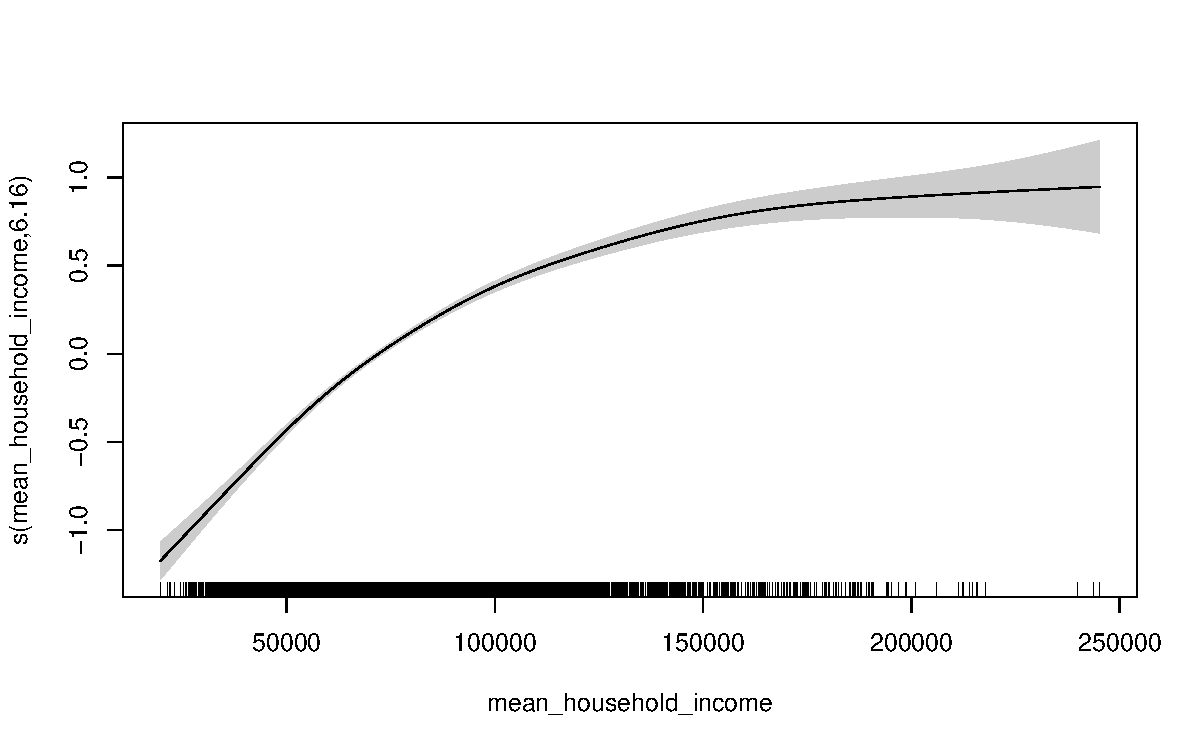
\includegraphics[width=\textwidth]{img/gamRug02.pdf}
\end{center}

\end{frame}

%%%%%%%%%%%%%%%%%%%%%%%%%%%%%%%%%%%%%%%%%%%%%%%%%%%
\begin{frame}[fragile] \frametitle{} \oldB \small

\begin{center}
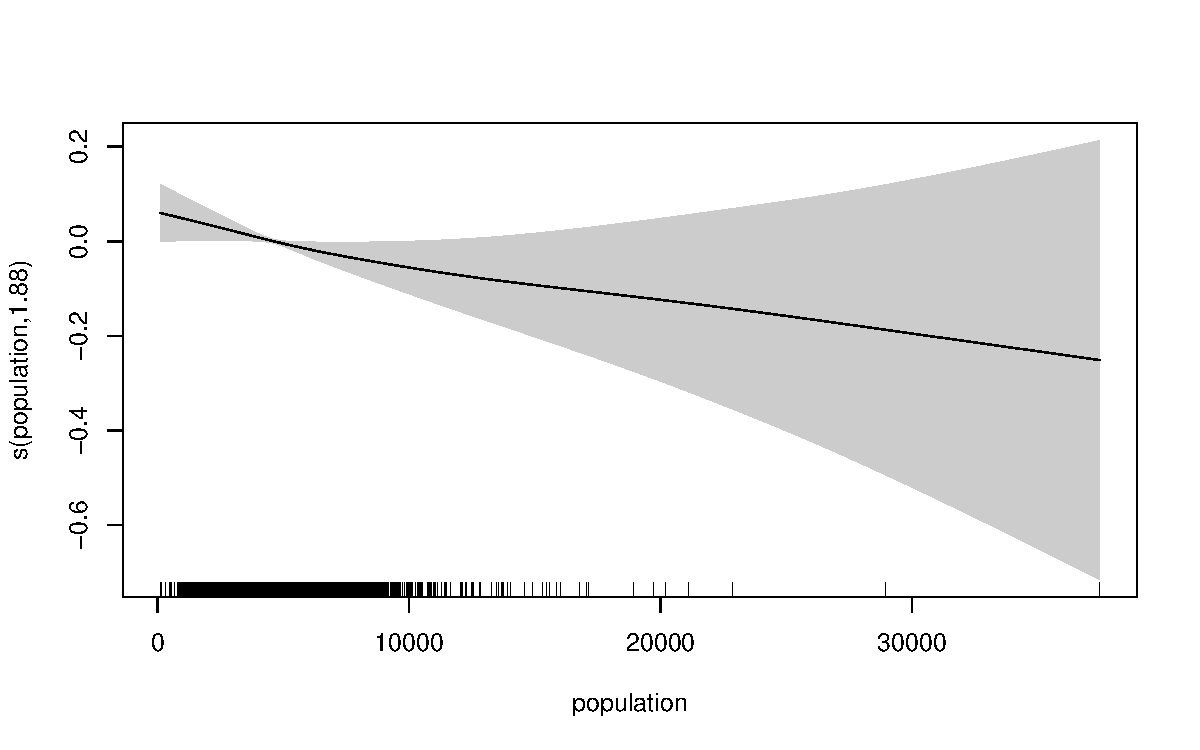
\includegraphics[width=\textwidth]{img/gamRug03.pdf}
\end{center}

\end{frame}

%%%%%%%%%%%%%%%%%%%%%%%%%%%%%%%%%%%%%%%%%%%%%%%%%%%
\begin{frame}[fragile] \frametitle{} \oldB \small

\begin{center}
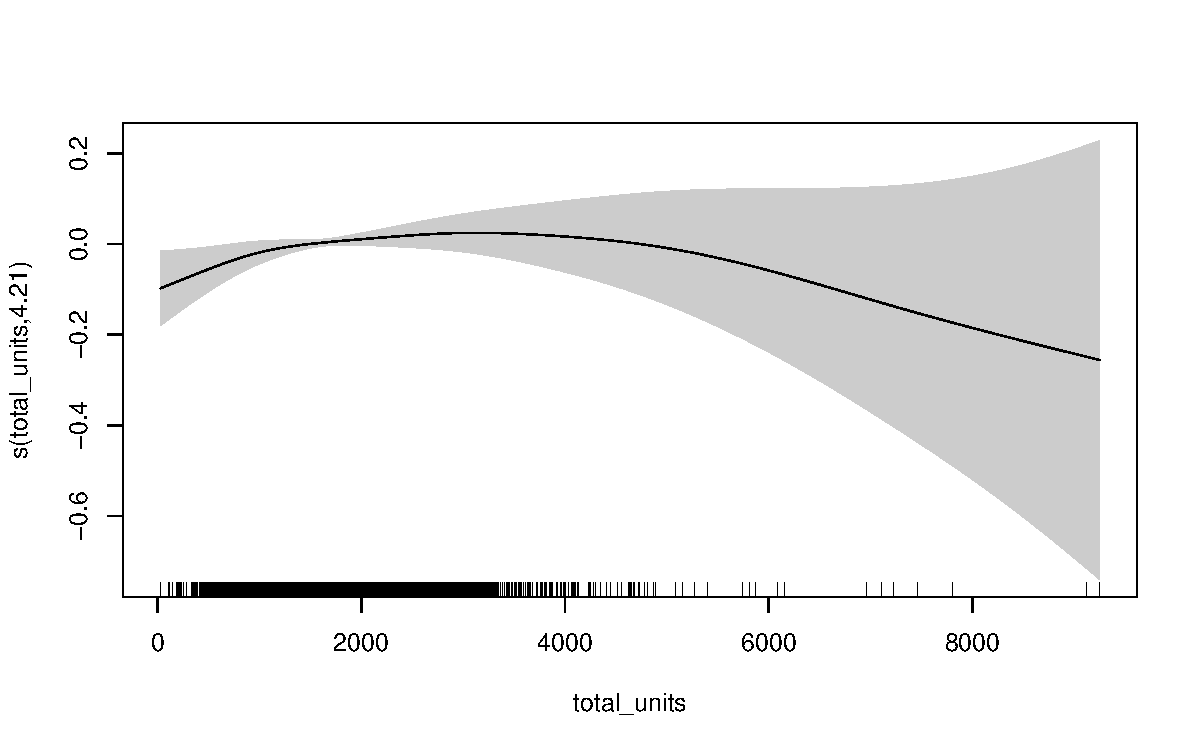
\includegraphics[width=\textwidth]{img/gamRug04.pdf}
\end{center}

\end{frame}

%%%%%%%%%%%%%%%%%%%%%%%%%%%%%%%%%%%%%%%%%%%%%%%%%%%
\begin{frame}[fragile] \frametitle{} \oldB \small

\begin{center}
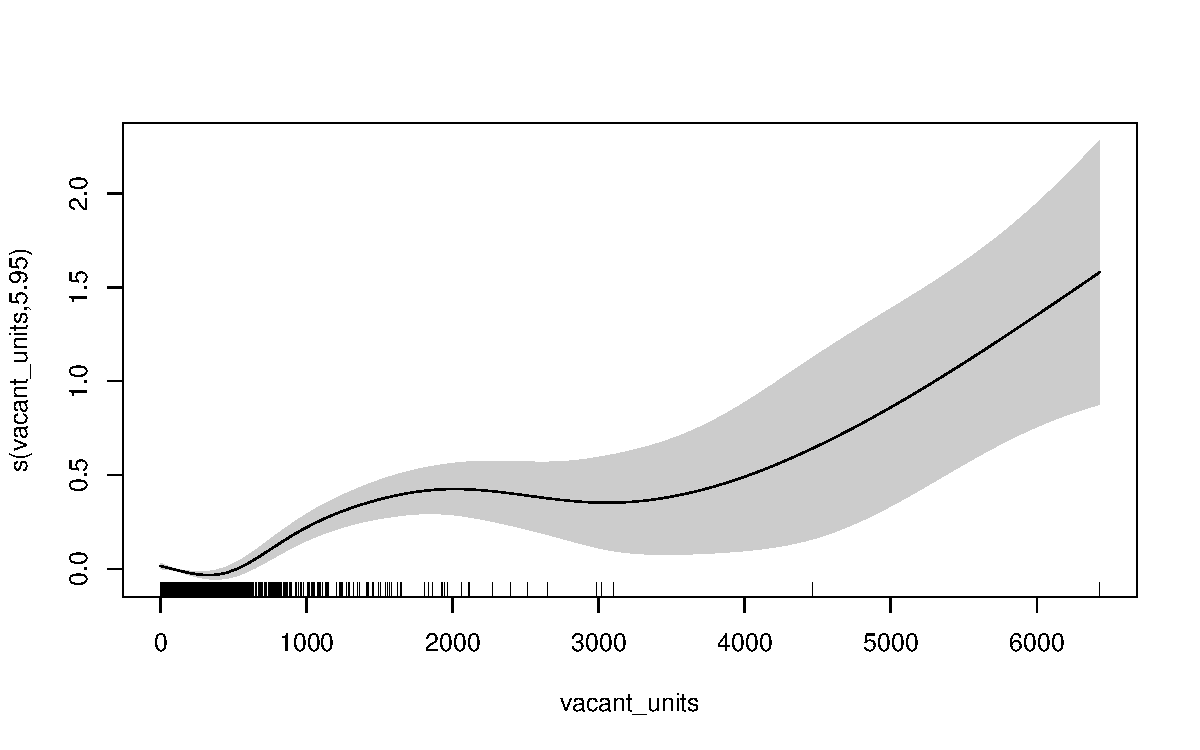
\includegraphics[width=\textwidth]{img/gamRug05.pdf}
\end{center}

\end{frame}

%%%%%%%%%%%%%%%%%%%%%%%%%%%%%%%%%%%%%%%%%%%%%%%%%%%
\begin{frame}[fragile] \frametitle{} \oldB \small

\begin{center}
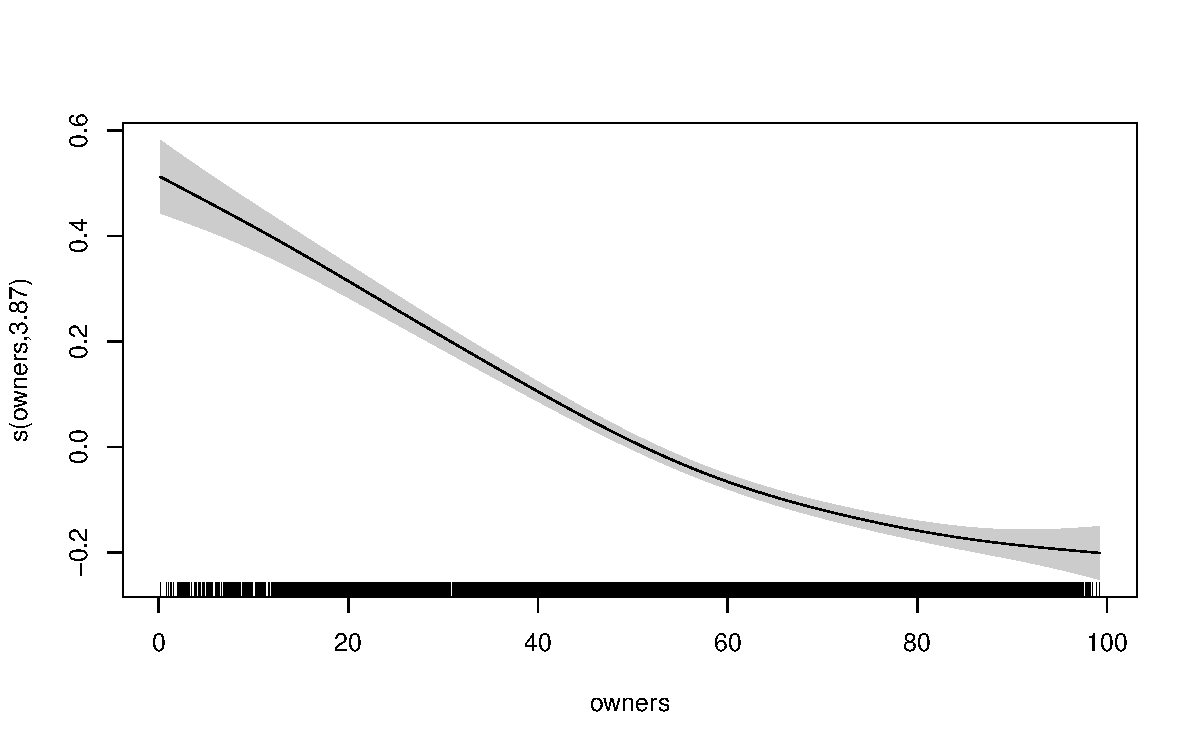
\includegraphics[width=\textwidth]{img/gamRug06.pdf}
\end{center}

\end{frame}

%%%%%%%%%%%%%%%%%%%%%%%%%%%%%%%%%%%%%%%%%%%%%%%%%%%
\begin{frame}[fragile] \frametitle{} \oldB \small

\begin{center}
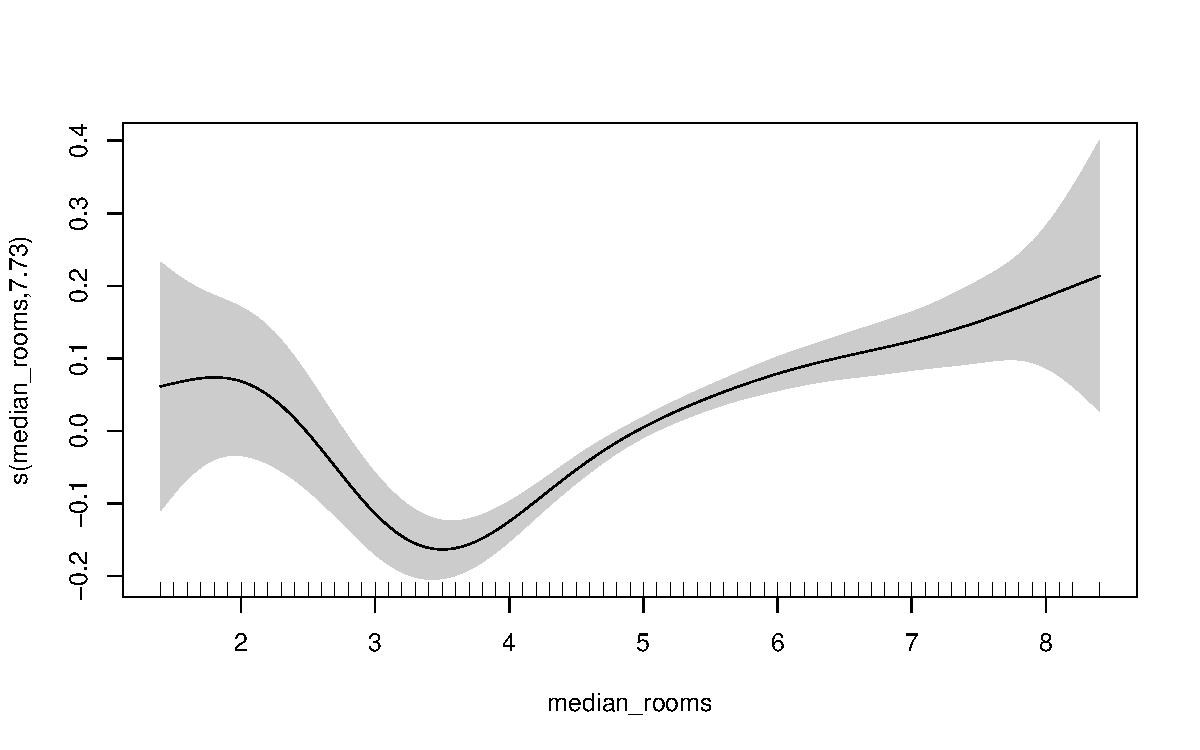
\includegraphics[width=\textwidth]{img/gamRug07.pdf}
\end{center}

\end{frame}

%%%%%%%%%%%%%%%%%%%%%%%%%%%%%%%%%%%%%%%%%%%%%%%%%%%
\begin{frame}[fragile] \frametitle{} \oldB \small

\begin{center}
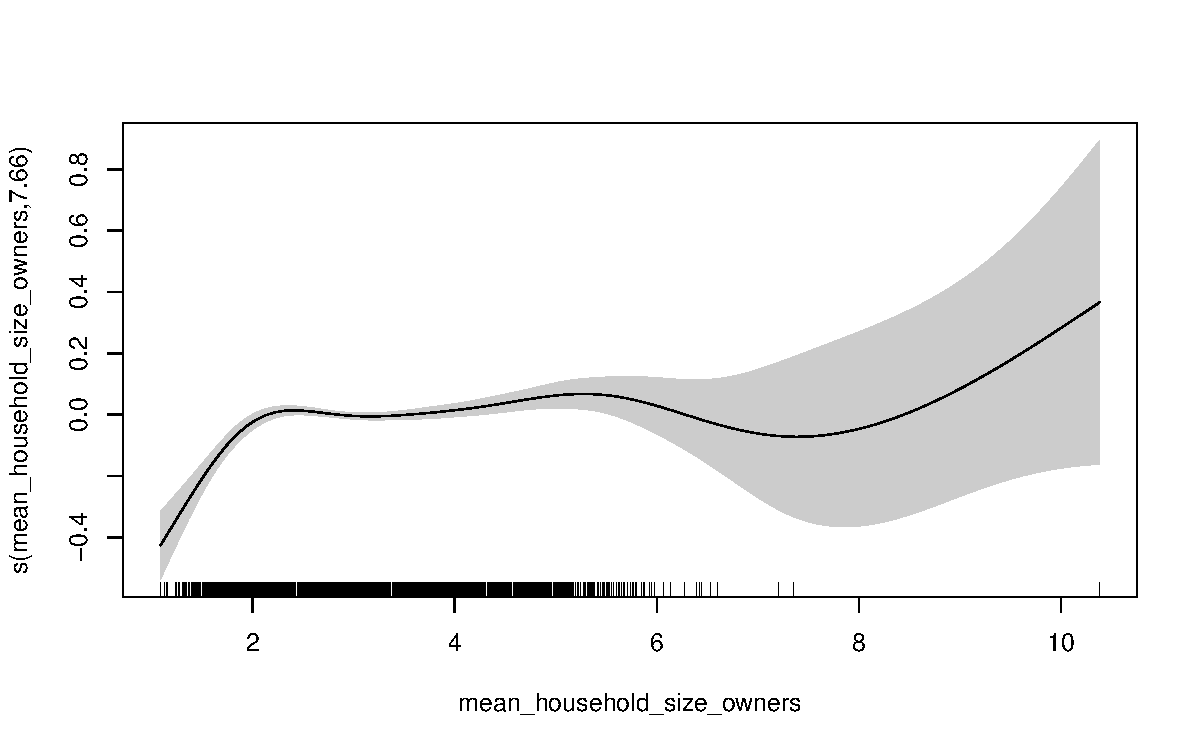
\includegraphics[width=\textwidth]{img/gamRug08.pdf}
\end{center}

\end{frame}

%%%%%%%%%%%%%%%%%%%%%%%%%%%%%%%%%%%%%%%%%%%%%%%%%%%
\begin{frame}[fragile] \frametitle{} \oldB \small

\begin{center}
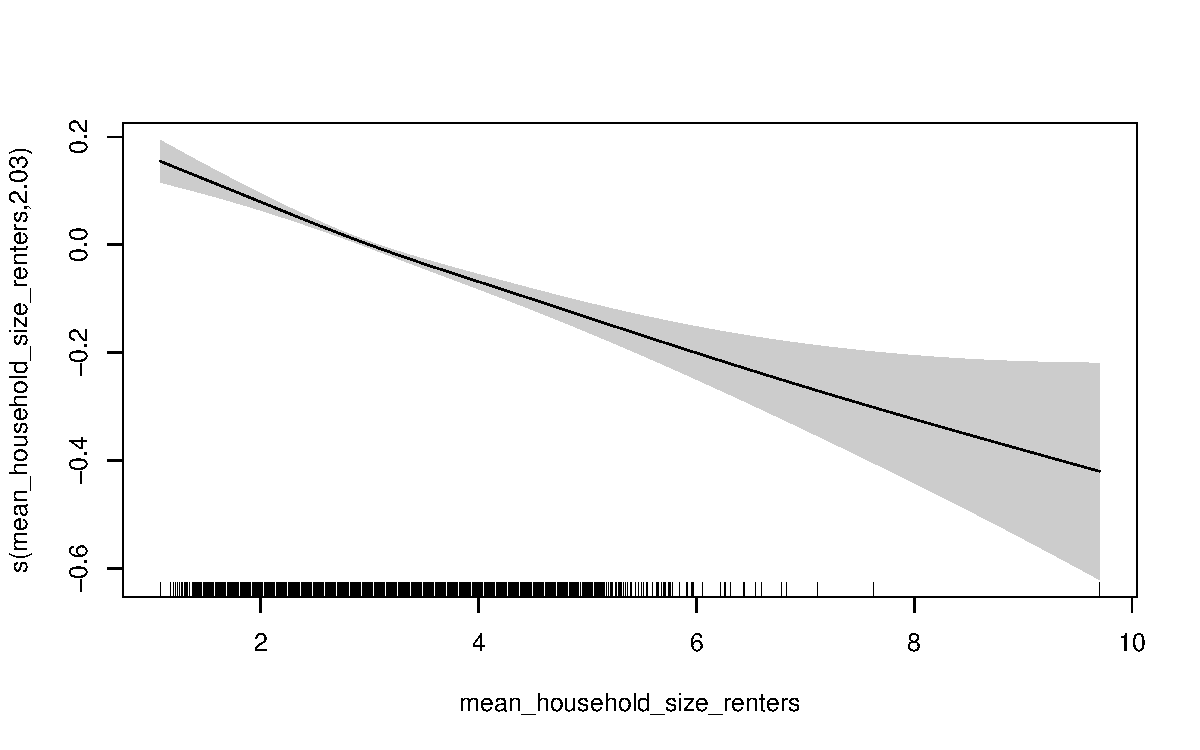
\includegraphics[width=\textwidth]{img/gamRug09.pdf}
\end{center}

\end{frame}

%%%%%%%%%%%%%%%%%%%%%%%%%%%%%%%%%%%%%%%%%%%%%%%%%%%
\begin{frame}[fragile] \frametitle{} \oldB \small

\begin{center}
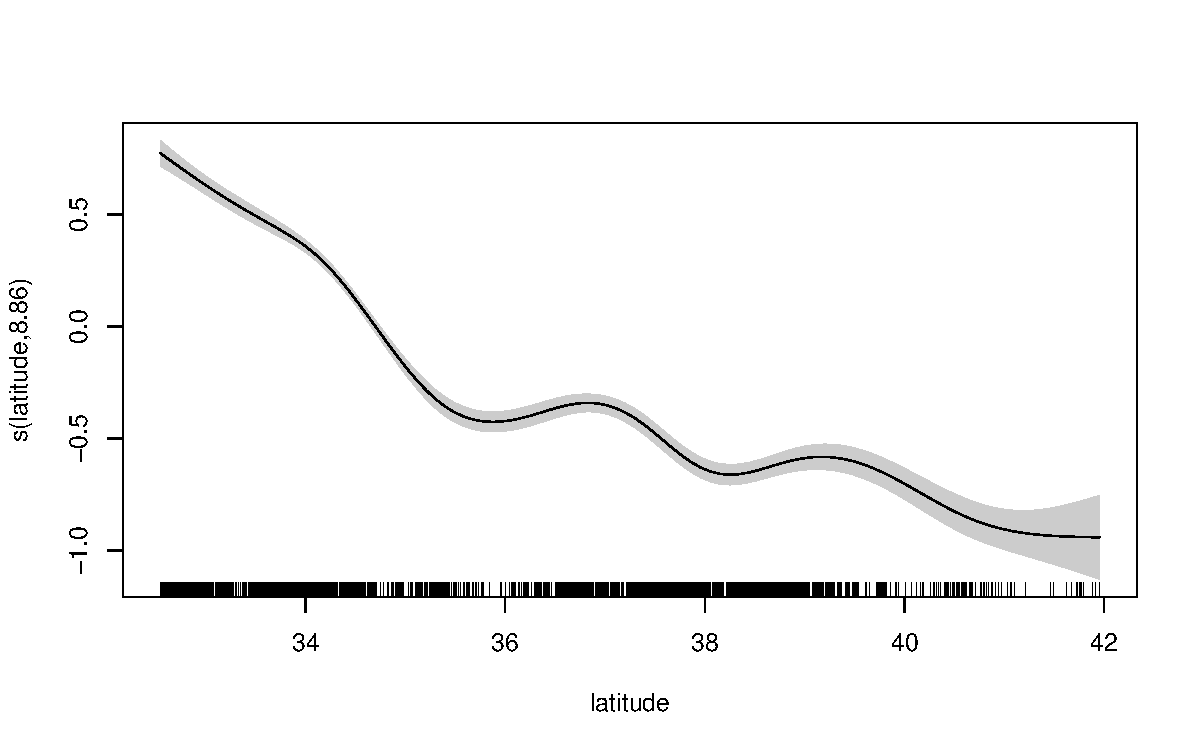
\includegraphics[width=\textwidth]{img/gamRug10.pdf}
\end{center}

\end{frame}

%%%%%%%%%%%%%%%%%%%%%%%%%%%%%%%%%%%%%%%%%%%%%%%%%%%
\begin{frame}[fragile] \frametitle{} \oldB \small

\begin{center}
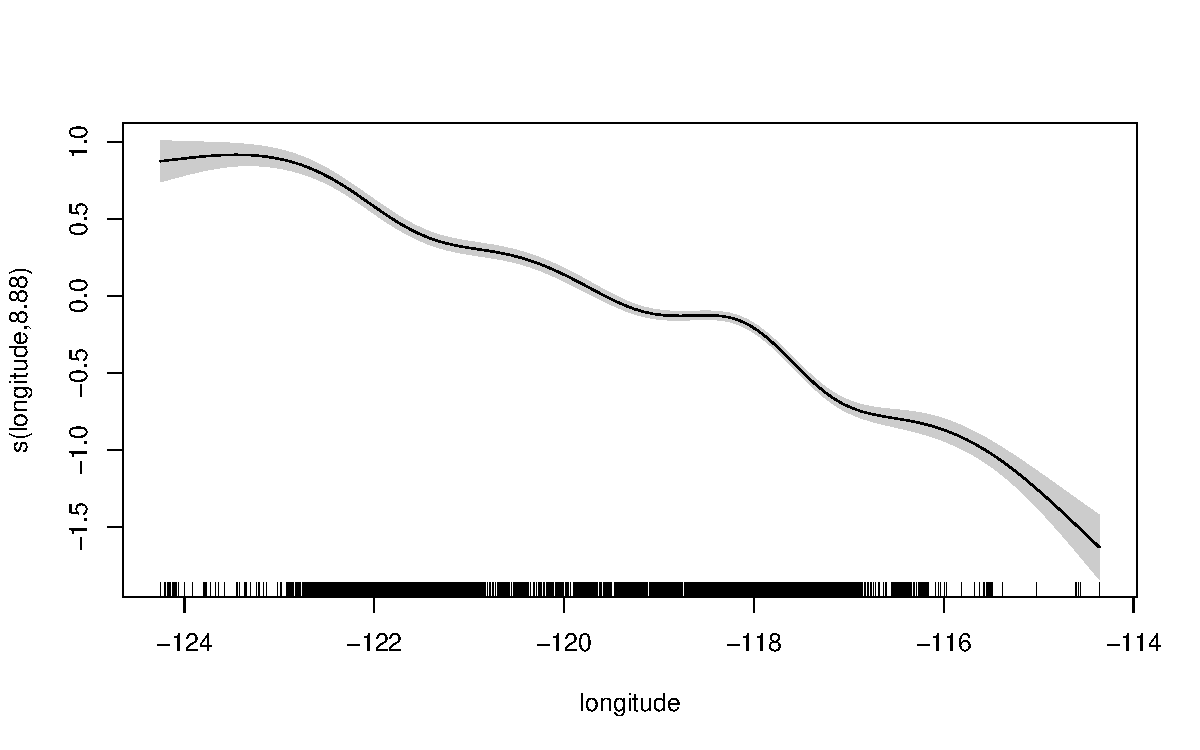
\includegraphics[width=\textwidth]{img/gamRug11.pdf}
\end{center}

\end{frame}

%%%%%%%%%%%%%%%%%%%%%%%%%%%%%%%%%%%%%%%%%%%%%%%%%%%
\begin{frame}[fragile] \frametitle{} \oldB \small

It actually makes more sense to allow and interaction between
latitude and longitude. This is also easy to include in \texttt{mgcv}:
\begin{lstlisting}[language=R, basicstyle=\fontsize{8pt}{10pt}\selectfont\ttfamily]
> ca.gam2 <- gam(log(median_house_value)
+   ~ s(median_household_income) + s(mean_household_income)
+   + s(population) + s(total_units) + s(vacant_units)
+   + s(owners) + s(median_rooms) + s(mean_household_size_owners)
+   + s(mean_household_size_renters)
+   + s(longitude,latitude), data=ca, subset=trainFlag)
\end{lstlisting}

\end{frame}

%%%%%%%%%%%%%%%%%%%%%%%%%%%%%%%%%%%%%%%%%%%%%%%%%%%
\begin{frame}[fragile] \frametitle{} \oldB \small

\begin{center}
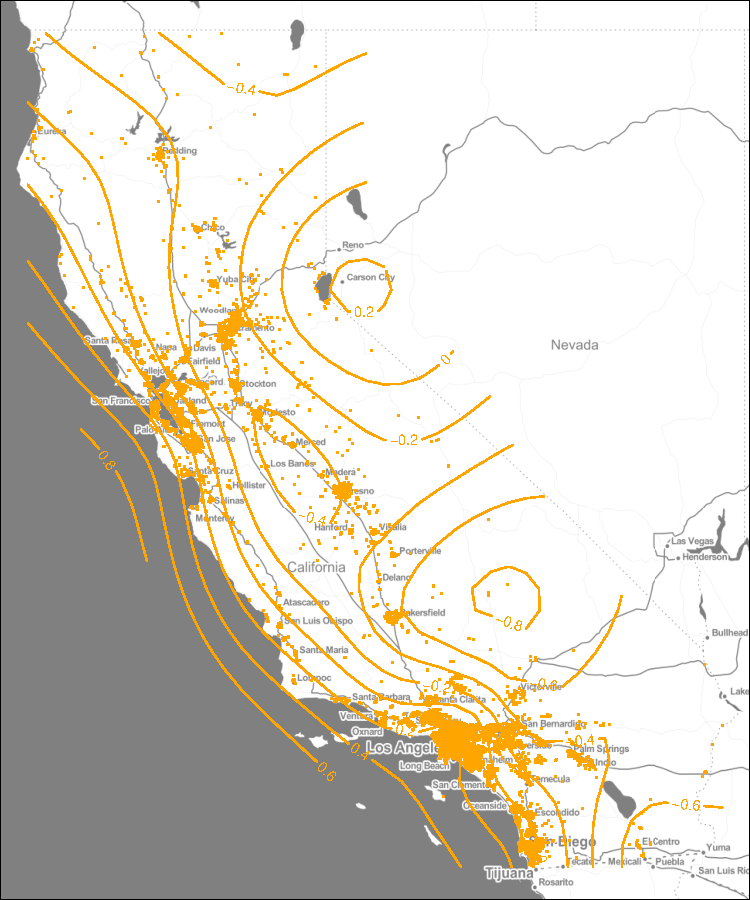
\includegraphics[height=\textheight]{img/fig03.pdf}
\end{center}

\end{frame}


%%%%%%%%%%%%%%%%%%%%%%%%%%%%%%%%%%%%%%%%%%%%%%%%%%%
\begin{frame}[fragile] \frametitle{} \oldB \small

How well does these methods do in terms of prediction? We can
predict using the \texttt{predict} function just as with linear
models:
\begin{lstlisting}[language=R, basicstyle=\fontsize{8pt}{10pt}\selectfont\ttfamily]
> y <- log(ca$median_house_value)
> ca.lm.pred <- predict(ca.lm, ca)
> ca.gam.pred <- predict(ca.gam, ca)
> ca.gam2.pred <- predict(ca.gam2, ca)
\end{lstlisting}
And then check the mean squared error on both the
training set and testing set:
\begin{lstlisting}[language=R, basicstyle=\fontsize{8pt}{10pt}\selectfont\ttfamily]
> tapply((ca.lm.pred - y)^2, trainFlag, mean)
FALSE  TRUE
0.096 0.101
> tapply((ca.gam.pred - y)^2, trainFlag, mean)
FALSE  TRUE
0.064 0.072
> tapply((ca.gam2.pred - y)^2, trainFlag, mean)
FALSE  TRUE
0.059 0.065
\end{lstlisting}

\end{frame}


%%%%%%%%%%%%%%%%%%%%%%%%%%%%%%%%%%%%%%%%%%%%%%%%%%%
\begin{frame}[fragile] \frametitle{} \oldB \small

In machine learning, you'll often hear the caveat that everything
depend on future values following \magenta{the same underlying model}.
I think we say that a lot, but forget to really think about it.
To illustrate, let's re-fit the model on the California data without
the latitude and longitude components. We can then see how well the
model trained on California data generalizes to Pennsylvania data.

\end{frame}

%%%%%%%%%%%%%%%%%%%%%%%%%%%%%%%%%%%%%%%%%%%%%%%%%%%
\begin{frame}[fragile] \frametitle{} \oldB \small

Here are the two linear models fit on the two different datasets.
\begin{lstlisting}[language=R, basicstyle=\fontsize{8pt}{10pt}\selectfont\ttfamily]
> ca.lm2 <- lm(log(median_house_value) ~ median_household_income
+   + mean_household_income + population + total_units +
+   + vacant_units + owners + median_rooms +
+   + mean_household_size_owners + mean_household_size_renters,
+   data = ca, subset=trainFlag)
>
> pa.lm3 <- lm(log(median_house_value) ~ median_household_income
+   + mean_household_income + population + total_units +
+   + vacant_units + owners + median_rooms +
+   + mean_household_size_owners + mean_household_size_renters,
+   data = pa, subset=trainFlag)
\end{lstlisting}

\end{frame}


%%%%%%%%%%%%%%%%%%%%%%%%%%%%%%%%%%%%%%%%%%%%%%%%%%%
\begin{frame}[fragile] \frametitle{} \oldB \small

And here are the two additive models fit on the data:
\begin{lstlisting}[language=R, basicstyle=\fontsize{8pt}{10pt}\selectfont\ttfamily]
> ca.gam3 <- gam(log(median_house_value)
+   ~ s(median_household_income) + s(mean_household_income)
+   + s(population) + s(total_units) + s(vacant_units)
+   + s(owners) + s(median_rooms) + s(mean_household_size_owners)
+   + s(mean_household_size_renters), data=ca, subset=trainFlagPa)
>
> pa.gam4 <- gam(log(median_house_value)
+   ~ s(median_household_income) + s(mean_household_income)
+   + s(population) + s(total_units) + s(vacant_units)
+   + s(owners) + s(median_rooms) + s(mean_household_size_owners)
+   + s(mean_household_size_renters), data=pa, subset=trainFlagPa)
\end{lstlisting}

\end{frame}

%%%%%%%%%%%%%%%%%%%%%%%%%%%%%%%%%%%%%%%%%%%%%%%%%%%
\begin{frame}[fragile] \frametitle{} \oldB \small

Fitting these models all on the PA data:
\begin{lstlisting}[language=R, basicstyle=\fontsize{8pt}{10pt}\selectfont\ttfamily]
> y.pa <- log(pa$median_house_value)
> pa.lm2.pred <- predict(ca.lm2, pa)
> pa.gam3.pred <- predict(ca.gam3, pa)
> pa.lm3.pred <- predict(pa.lm3, pa)
> pa.gam4.pred <- predict(pa.gam4, pa)
\end{lstlisting}
We see that the California ones yield very poor MSE scores
for PA:
\begin{lstlisting}[language=R, basicstyle=\fontsize{8pt}{10pt}\selectfont\ttfamily]
> tapply((pa.lm2.pred - y.pa)^2,trainFlagPa,mean)
FALSE  TRUE
 0.58  0.55
> tapply((pa.gam3.pred - y.pa)^2,trainFlagPa,mean)
FALSE  TRUE
 0.47  0.44
> tapply((pa.lm3.pred - y.pa)^2,trainFlagPa,mean)
FALSE  TRUE
0.095 0.093
> tapply((pa.gam4.pred - y.pa)^2,trainFlagPa,mean)
FALSE  TRUE
0.070 0.063
\end{lstlisting}

\end{frame}


%%%%%%%%%%%%%%%%%%%%%%%%%%%%%%%%%%%%%%%%%%%%%%%%%%%
\begin{frame}[fragile] \frametitle{} \oldB \small

If we account for the overall means being different, we
see that the California models perform reasonably well on
the Pennsylvania data:
\begin{lstlisting}[language=R, basicstyle=\fontsize{8pt}{10pt}\selectfont\ttfamily]
> tapply((pa.lm2.pred - y.pa),trainFlagPa,var)
FALSE  TRUE
 0.14  0.13
> tapply((pa.gam3.pred - y.pa),trainFlagPa,var)
FALSE  TRUE
0.094 0.084
> tapply((pa.lm3.pred - y.pa),trainFlagPa,var)
FALSE  TRUE
0.095 0.093
> tapply((pa.gam4.pred - y.pa),trainFlagPa,var)
FALSE  TRUE
0.070 0.063
\end{lstlisting}

\end{frame}





\end{document}













